\documentclass{standalone}
\usepackage{pgfplots}
\usetikzlibrary{intersections}
\pgfplotsset{compat=1.7}

\begin{document}
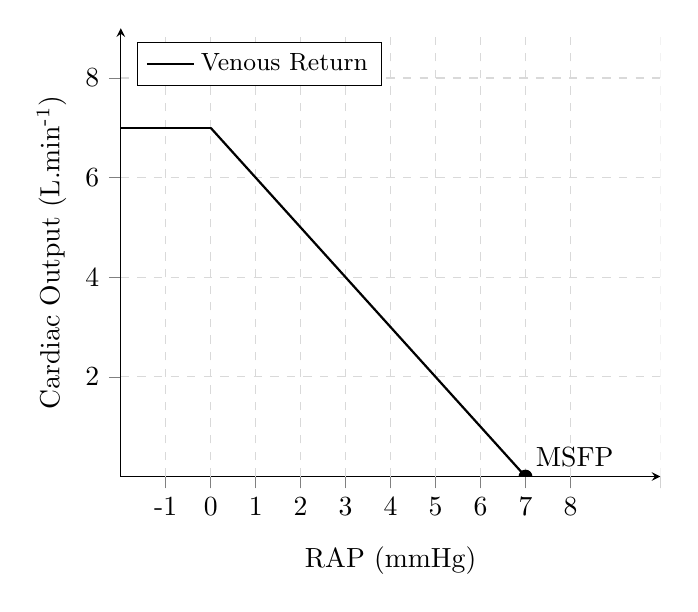
\begin{tikzpicture}


\begin{axis}[
        axis lines=middle,
        grid = major,
        grid style={dashed, gray!30},
	ymin = 0,
	ymax = 9,
	xmin = 0,
	xmax =12,
	 ylabel near ticks,
	xlabel near ticks,
	xticklabels={},
	extra x ticks={1,2,3,4,5,6,7,8,9,10},
	extra x tick labels={-1,0,1,2,3,4,5,6,7,8,9,10},
        xlabel=RAP (mmHg),
        ylabel=Cardiac Output (L.min\textsuperscript{-1}),
        tick align=outside,
        enlargelimits=false,
legend pos= north west,
legend style={font=\small, cells={align=left}}]

\draw[name=vr, black, thick] (axis cs: 0, 7) -- (axis cs: 2,7);
\plot[domain=2:9, black, thick,samples=500] {9-x} node[pos=1,circle,fill=black,inner sep=0pt,minimum size=5pt]{} node[pos=1, above right]{MSFP};
\addlegendentry{Venous Return}




\end{axis}

\end{tikzpicture} 
\end{document}